% !TEX root = ./main.tex
% !TEX encoding = UTF-8 Unicode
% !TEX program = pdflatex
% !TeX spellcheck = it_IT

\chapter{Studio preliminare del dataset}
Il dataset iniziale è fornito di 5 differenti files in formato "\textbf{json}":
\begin{itemize}
	\item \textbf{User}: contiene informazioni riguardanti gli utenti iscritti e le loro amicizie (circa 1.1M);
	\item \textbf{Business}: contiene informazioni riguardanti i business recensiti (circa 144K);
	\item \textbf{Review}: contiene le recensioni che gli utenti hanno effettuato per i business (circa 4.1M);
	\item \textbf{Checkin}: contiene informazioni riguardanti le visite effettuate nel tempo presso i differenti business;
	\item \textbf{Tip}: contiene informazioni riguardanti i suggerimenti che gli utenti hanno lasciato ai differenti business.
\end{itemize}

\'E stata effettuata un'analisi preliminare del problema andando direttamente ad
utilizzare la piattaforma, al fine di comprenderne meglio le dinamiche di
funzionamento.\\
In particolare, ogni utente iscritto possiede una propria
pagina personale, sulla quale altri utenti possono lasciare differenti
"\textit{complimenti}".\\
Ogni utente può lasciare una recensione ed un punteggio in
\textbf{stars} ad un business che ha visitato.\\
Ogni recensione, a sua volta, può essere giudicata dagli altri utenti con tre
differenti reazioni:
\begin{itemize}
	\item \textbf{Funny};
	\item \textbf{Useful};
	\item \textbf{Cool}.
\end{itemize}
Yelp utilizza anche un criterio per definire influenti o meno i suoi utenti iscritti,
assegnando il titolo di "\textit{elite}".\\

\section{Analisi in Power BI}
Al fine di calpire al meglio le caratteristiche dei dati e, soprattutto, come
utilizzarli allo scopo della \textbf{Influence Maximization}, si è deciso di
effettuare un'analisi preliminare utilizzando un tool di \texttt{BI}.\\

\subsubsection{Review Count for User}
Nel dataset è presente, per ogni User, un attributo che esprime il numero di
recensioni realizzate a partire dalla loro data di iscrizione.\\
\'E stato realizzato un report che controllasse che la somma dei numeri  delle
recensioni degli user corrispondesse effettivamente al numero di recensioni
presenti nel dataset \textit{Review}.\\
Questo è risultato falso, infatti non sono presenti tutte le recensioni
realmente effettuate da ogni user.\\
Questo rende tale attributo inutilizzabile per il nostro scopo.\\

\begin{figure}[!htbp]
	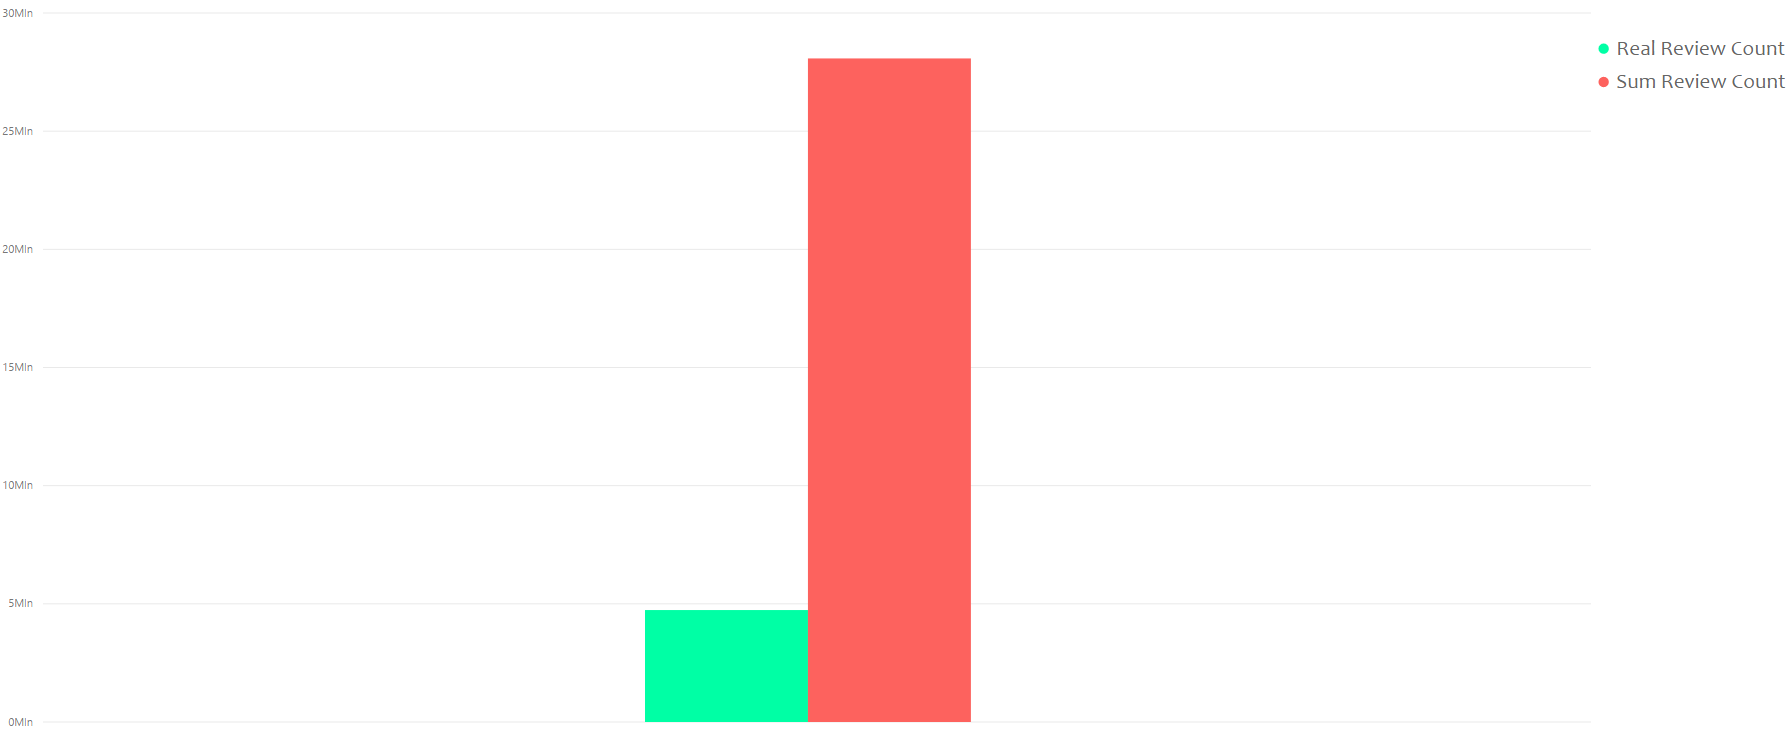
\includegraphics[width=1\linewidth,keepaspectratio]{review_count}
	\caption{Real Review Counts}
	\label{review_count}
\end{figure}

\subsubsection{Yearly Review Count}
\'E stato fondamentale, per l'analisi implementata, ricavare l'informazione riguardante la distribuzione delle
recensioni nei vari anni, dal 2004 ad oggi.\\
Il seguente report mostra, appunto, tale trend:\\

\begin{figure}[!htbp]
	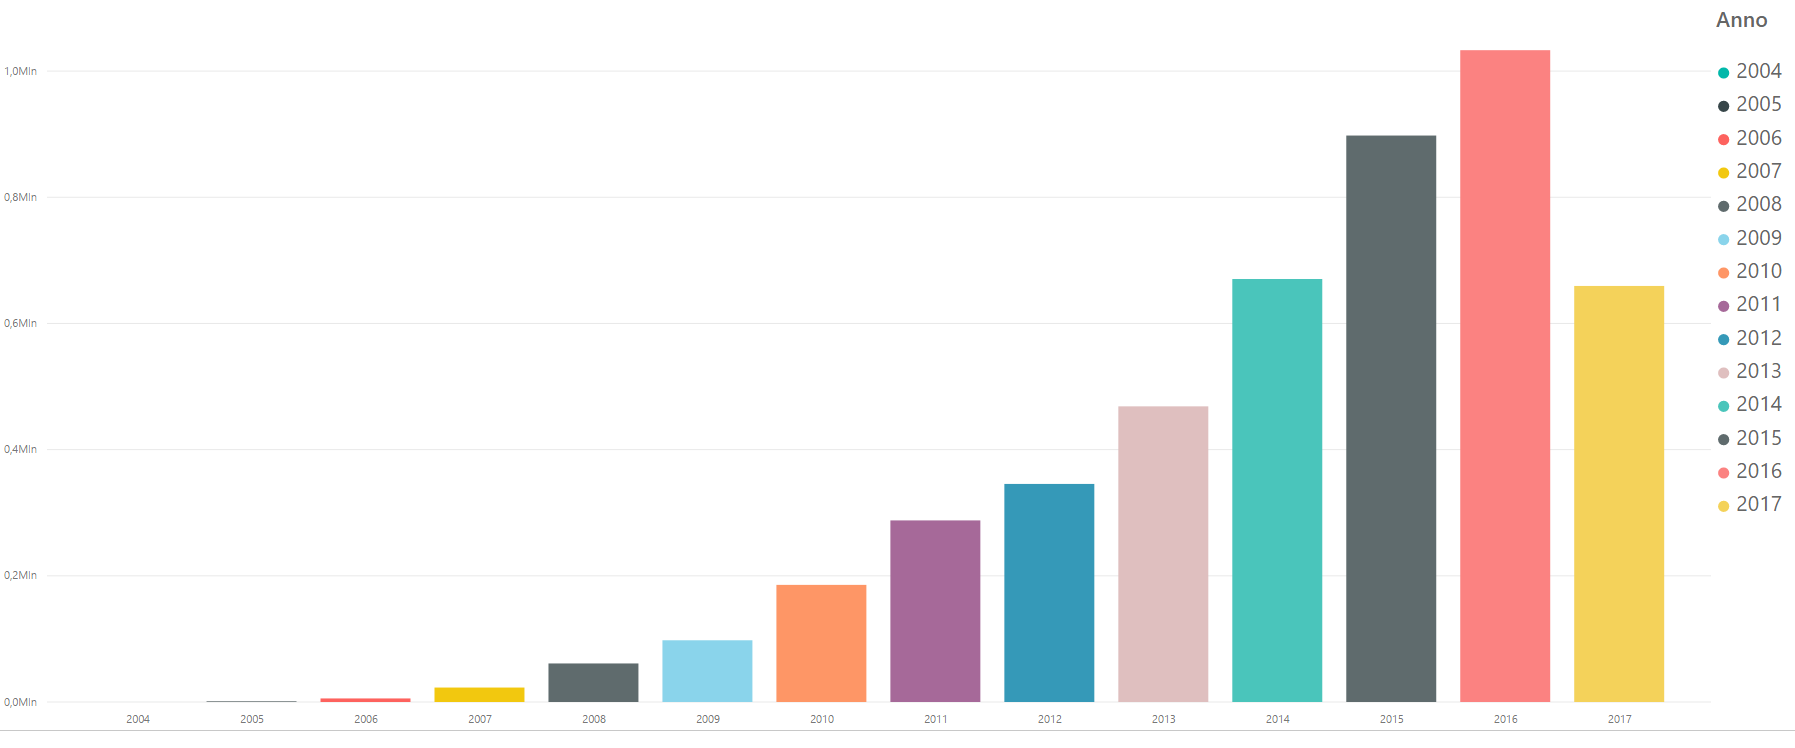
\includegraphics[width=1\linewidth,keepaspectratio]{review_count_anno}
	\caption{Yearly Review Counts}
	\label{review_count_anno}
\end{figure}

\clearpage

\subsubsection{Monthly Reviews Trend}
Essendo un problema di \textit{Influence Maximization}, si è pensato di
considerare solo gli utenti definibili come ``\textit{attivi}'' negli ultimi anni.\\
Per fare ciò è stato necessario visualizzare, per ogni mese, la percentuale, sul
totale, di recensioni effettuate, così da decidere di effettuare una scrematura
delle recensioni in funzione della loro data.

\begin{figure}[!htbp]
	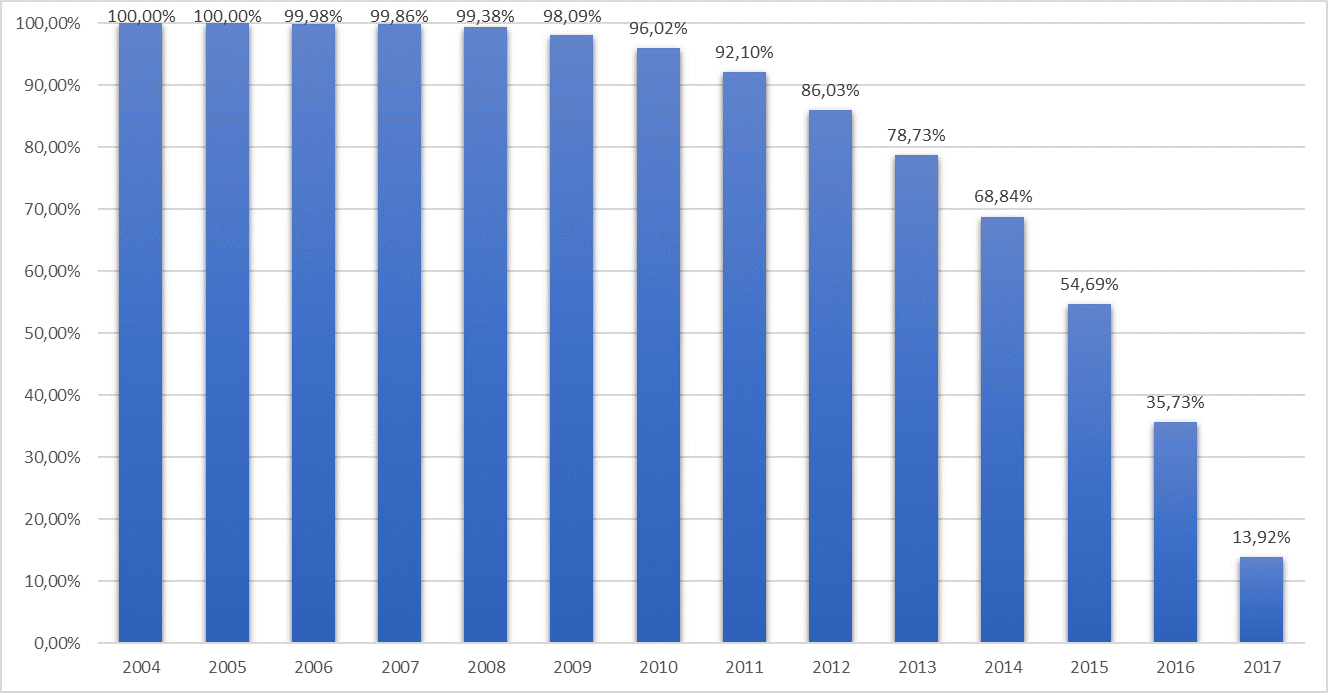
\includegraphics[width=1\linewidth,keepaspectratio]{yearly_monthly_choice}
	\caption{Monthly Reviews Trend}
	\label{yearly_monthly_choice}
\end{figure}

\begin{figure}[!htbp]
	\centering
	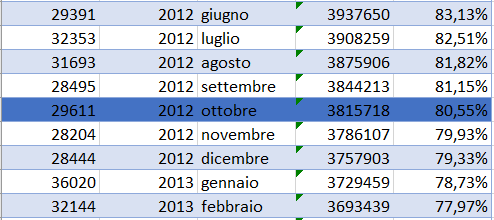
\includegraphics[width=.9\linewidth,keepaspectratio]{table_yearly_monthly_choice}
	\caption{Table Monthly Reviews Trend}
	\label{table_yearly_monthly_choice}
\end{figure}

Si è deciso di considerare solo le recensioni successive all'\textbf{Ottobre 2012},
assicurando la copertura dell'80.55\% del dataset iniziale.\\

\clearpage

\subsubsection{Users with more Reviews}
Una prima ricerca di utenti più influenti può essere effettuata individuando
gli utenti che hanno realizzato più recensioni sulla piattaforma \textit{Yelp}.

\begin{figure}[!htbp]
	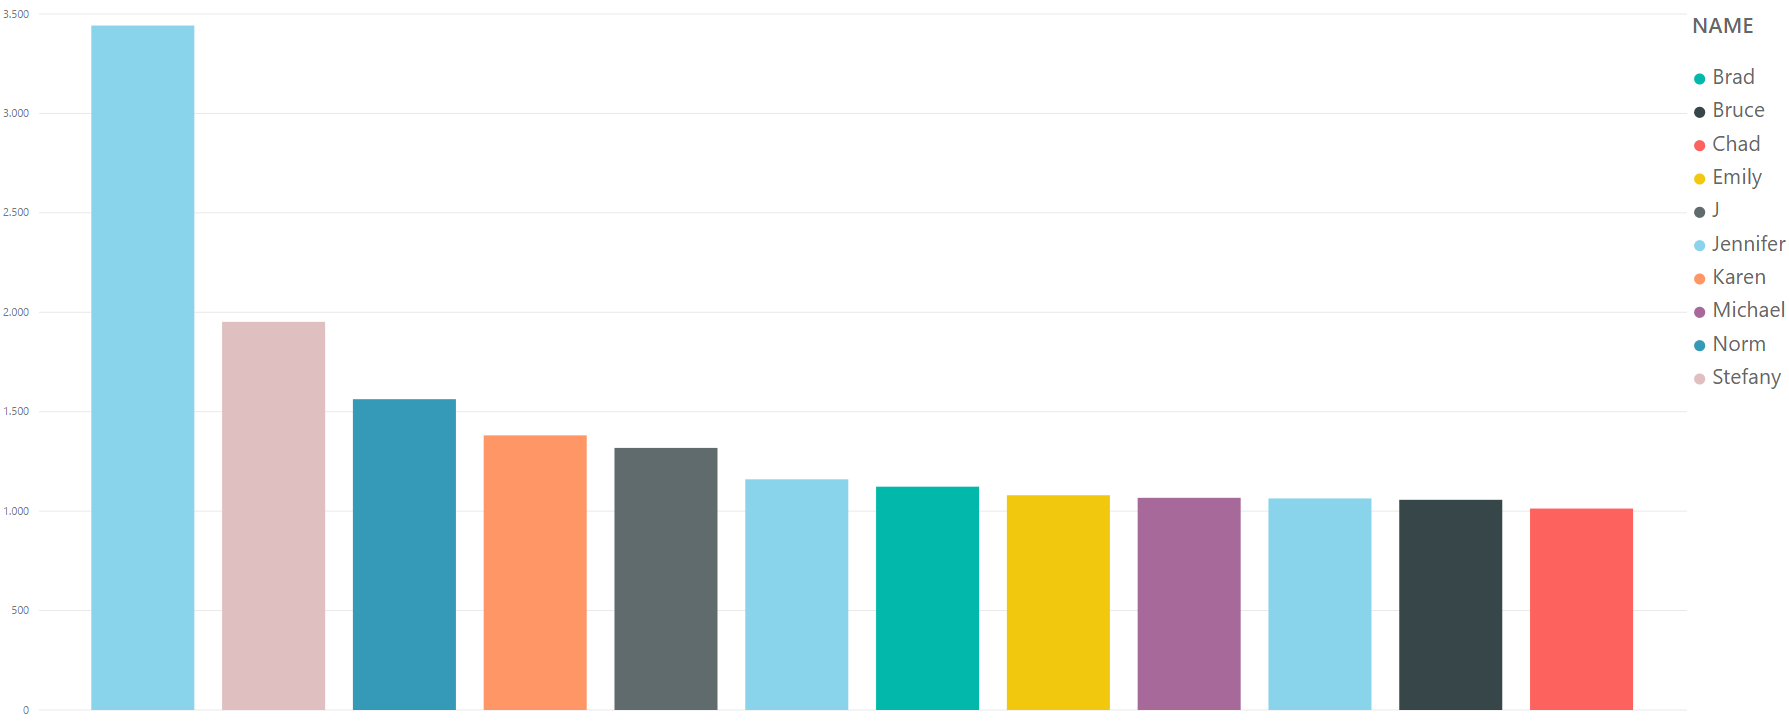
\includegraphics[width=1\linewidth,keepaspectratio]{10_user_most_reviews}
	\caption{10 Users with more Reviews}
	\label{10_user_most_reviews}
\end{figure}
